\chapter{Otros proyectos libres similares}

A continuación podremos ver algunos de los proyectos que podemos encontrar por \textit{\textbf{Github}} sobre la generación automatizada de horarios.

\section{Plan}

\href{https://github.com/adamcik/plan}{\textit{Plan}} es un software desarrollado como asistente para la creación de horarios de una forma fácil para los estudiantes de \textit{NTNU}, tal y como se puede ver en \cite{plan}.

Esta interfaz web nos pide que creemos un \textit{nick} para poder entrar en la aplicación. Una vez creado, nos pasará a la interfaz que vemos en la \hyperref[plan1]{Figura \ref{plan1}}

\begin{figure}[H]
    \centering
    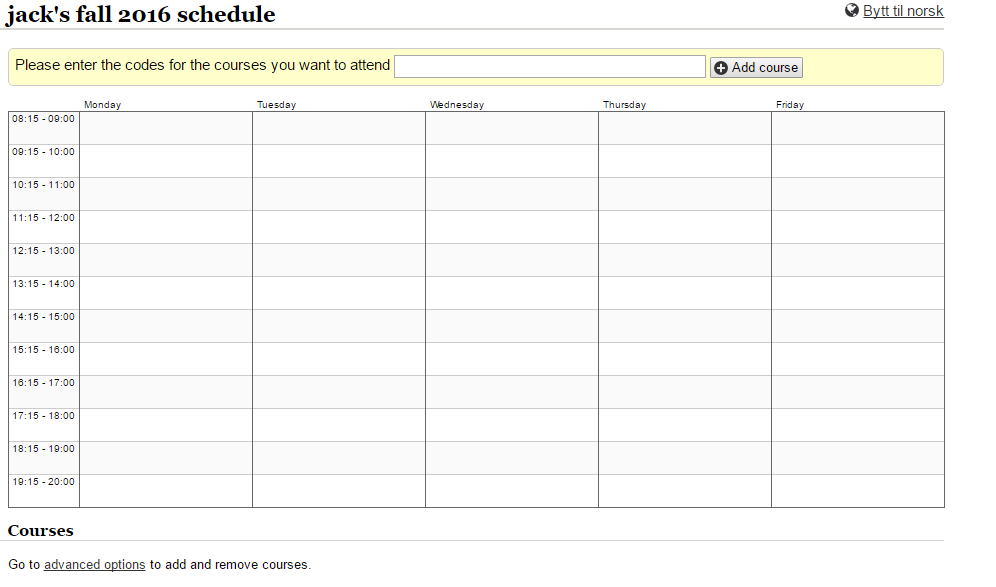
\includegraphics[width=0.7\textwidth]{plan1}
    \label{plan1}
    \caption{Interfaz web para la introducción de las asignaturas}
\end{figure}

En esta interfaz web, tendremos que ir introduciendo los códigos de las asignaturas, generando una tabla de asignaturas en la que el alumno se habrá matriculado, tal y como se puede ver en la \hyperref[plan2]{Figura \ref{plan2}}. En esta tabla, aparecerán los códigos de las asignaturas, su descripción, su fecha de examen y ofrece la posibilidad de dar un alias a la asignatura.

\begin{figure}[H]
    \centering
    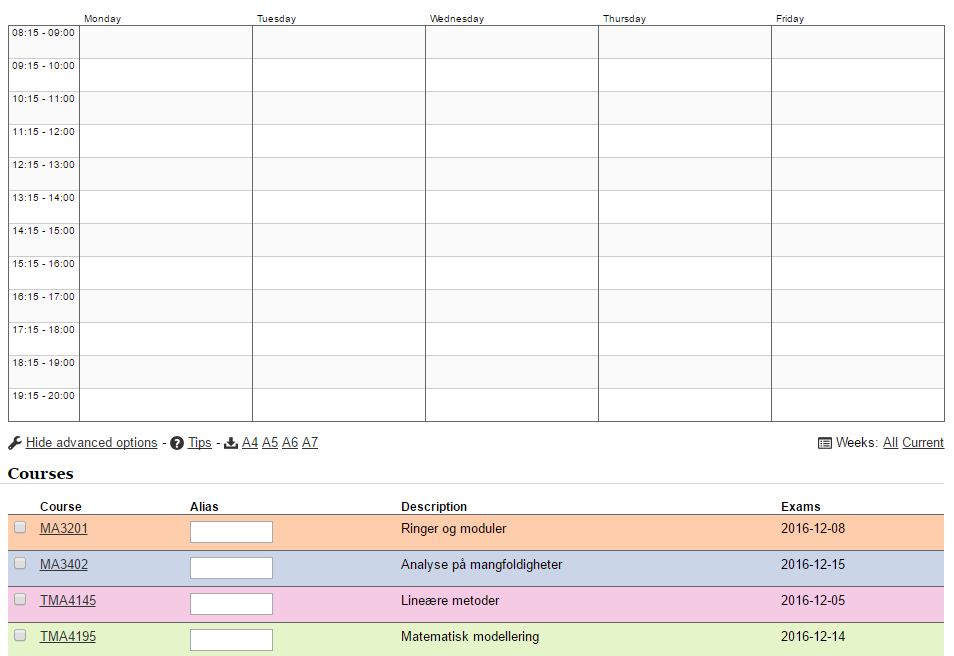
\includegraphics[width=0.7\textwidth]{plan2}
    \label{plan2}
    \caption{Tabla de asignaturas introducidas con sus respectivos códigos}
\end{figure}

Una vez introducidas, el alumno seleccionará los grupos en los que está matriculado y el sistema mostrará automáticamente \textbf{el horario específico para el alumno}. Es decir, dado un alumno con un conjunto de asignaturas $\mathcal{X}$, el sistema mostrará el horario que tiene el alumno en cuestión, como vemos en la \hyperref[plan3]{Figura \ref{plan3}}. A su vez, el sistema ofrece una lista con las clases de cada asignatura y grupo más detallada, como se ve en la \hyperref[plan4]{Figura \ref{plan4}}


\begin{figure}[H]
    \centering
    \mbox {
        
        \subfigure[Horario generado.]{
            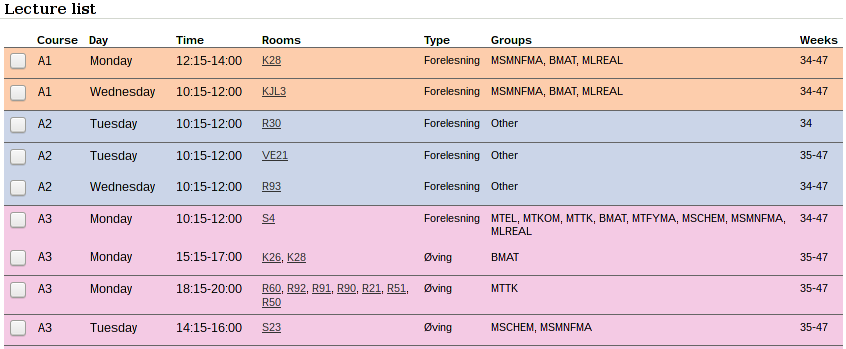
\includegraphics[width=0.5\textwidth]{plan3}
            \label{plan3}
        }
        
        \quad
        
        \subfigure[Lista más detallada de las clases del día.] {
            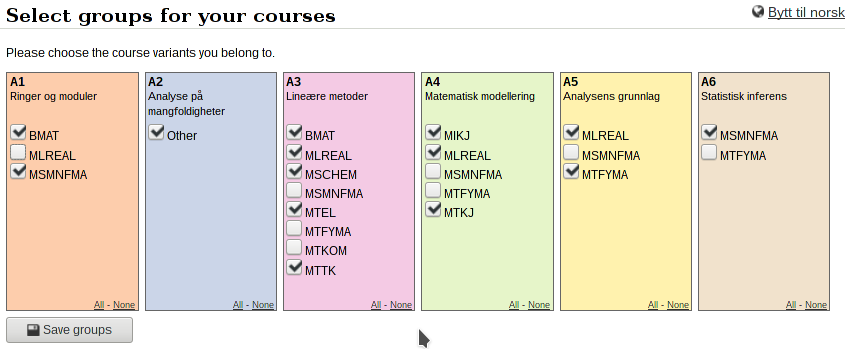
\includegraphics[width=0.5\textwidth]{plan4}
            \label{plan4}
        }
    }
    
    \caption{Horarios y listas que genera el sistema}
    \label{plan3-4}
\end{figure}

Este software ofrece actuálmente varias funciones tales como:

\begin{enumerate}
	\item Una vista personificable del calendario.
	\item Se puede exportar fácilmente a \textit{Google-Calendar}.
	\item Se puede imprimir en formato PDF.
	\item El usuario puede decidir las horas límites.
	\item Permite importar información sobre las asignaturas medianto volcados de una base de datos.
\end{enumerate}

\section{Timetable Generator}

\href{https://github.com/zeus9/timetable_generator}{\textit{Timetable Generator}} es un generador de horarios desarrollado por el usuario \textbf{zeus9} de \textit{Github}. Está desarrollado en C++ y Python 2, haciendo uso de un algoritmo genético para la generación del horario, tal y como se puede ver en \cite{timetableGenerator}.

Este sistema toma como entrada tres ficheros en formato \textbf{\textit{CSV}}, en los que se incluye la siguiente información:

\begin{enumerate}[$\bullet$]
    \item \texttt{initial.csv}: consiste en un fichero que contiene una matriz inicial que conforma el horario. Este horario inicial se utiliza en el algoritmo genético del fichero \textit{labGa.cpp}.
    \item \texttt{periodcount.csv}: supone una relación entre los $ID's$ de los profesores, disponibles en \textit{faculty.csv} y algo más aún por descifrar.
    \item \texttt{labPeriodcount.csv}
\end{enumerate}

Todo esto conforman los datos mínimos de la universidad que necesita el algoritmo para generar el horario. 

Para ejecutar el algoritmo, tiene que ser bajo una distribución Linux, y se realiza ejecutando en un terminal \texttt{./ttgen.sh}. Con esto, aparecerá en pantalla una interfaz muy simple que nos permite configurar los parámetros de ambos algoritmos como se ven en la \hyperref[ttgen1]{Figura \ref{ttgen1}}.

\begin{figure}[H]
    \centering
    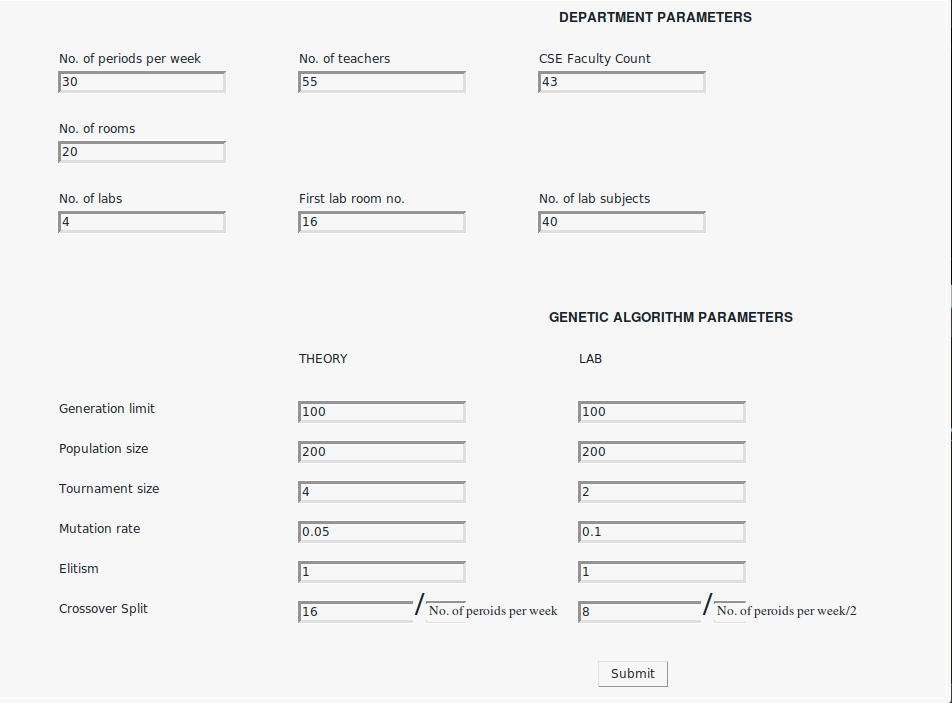
\includegraphics[width=0.7\textwidth]{ttgen1}
    \label{ttgen1}
    \caption{Interfaz para modificar los parámetros del algoritmo genético}
\end{figure}

Tras modificar los parámetros del algoritmo y pulsar el botón \textit{Submit}, estos datos se escriben en el fichero \textit{variables.csv} para el algoritmo genético de \textit{ga.cpp} y en \textit{labVariables.csv} para el algoritmo de \textit{labGa.cpp} y se comienza a ejecutar el $script$ en Python \texttt{labConflictsGen.py} que genera un CSV con las incompatibilidades que pueda haber en las aulas.